\gosam{} can be used either as a standalone code producing one-loop 
(and tree level) amplitudes, or it can be used as a \textit{One Loop Provider} (OLP)
in combination with a Monte Carlo program. 
The usage in the latter case is described in detail in Section \ref{sec:blha}. 
Below we will first describe the setup for the standalone version.


In order to generate the matrix element for a given process, the user should
create a process specific setup file, which we call {\em process card}. There
are no restrictions on the possible names or filename extensions, but the file
must be in plain ASCII format. For historical reasons \gosam process cards often
use the file extensions \texttt{*.in} or \texttt{*.rc}.

All possible options of the process card are given in Appendix~\ref{chp:process_card_options} with descriptions for each option.
The only mandatory fields are the \texttt{in} and \texttt{out} 
particles, the perturbative order and the path where to store the process files.
Therefore, a {\em minimal process card} can look like this:
\renewcommand*\thelstnumber{{\the\value{lstnumber}}}
\begin{lstlisting}[gobble=3,%
     numbers=left,caption={\texttt{eett.in}},%
     basicstyle=\ttfamily]
1  process_path=eett
2  in=    e+, e-
3  out=   t, t~
4  order= QCD, 0, 2
\end{lstlisting}


\section{Usage Example: \texorpdfstring{$e^+e^-\rightarrow t\bar{t}$}{e+e- to tt-bar}
at NLO in QCD}
\label{sec:usage}

In the following example we consider the calculation of the virtual QCD corrections to the process $e^+e^-\rightarrow t\bar{t}$. The process is defined in the following process card, which is a more realistic version of the minimal one given above.

\begin{lstlisting}[
     numbers=left,caption={\texttt{eett.rc}}, label={lst:eett},%
     basicstyle=\ttfamily] 
process_name=eett
process_path=virtual
in=-11,11
out=6,-6
order=QCD, 0, 2
one=gs,e
zero=wT,me
filter.particles=H:0,chi:0
reduction_programs=ninja,golem95
\end{lstlisting}
\renewcommand*\thelstnumber{\$}
Here only options differing from the default values are shown. The full list of options and their respective descriptions is available in Appendix~\ref{chp:process_card_options}.

The first two lines define the name and path of the produced process library, after which the actual process definition is given in lines 3-5. Most notably, this includes the coupling order definition in line 5. This statement restricts the order in the given coupling for the tree-level and one-loop diagrams respectively. Here, \texttt{QCD, 0, 2} specifies the tree-level diagrams to be of order $g_S^0$ and the one-loop diagrams to be of order $g_S^2$. No order of $g_W$ or $e$ is specified in this example, therefore both types of diagrams will be at leading order in the electroweak couplings.
The following options, lines 6 to 8, set some more properties of the process. Both coupling constants are set to unity symbolically, which is done by specifying them in the option \texttt{one}. This is useful if the couplings are multiplied later on as overall factors, typically by the Monte Carlo program. In the next line, the width of the top is set to zero, as is the mass of the electron. The \texttt{filter.particles} statement in line~8 suppresses the generation of diagrams with internal Higgs or Goldstone boson propagators. This is in principle not necessary, since those diagrams will all evaluate to zero for vanishing electron mass, but by setting the filter the respective diagrams will be discarded right from the start. Finally, the last line specifies which reduction backends the generated process library will support. Here, both supported backends are enabled. In such a case, the default reduction method at runtime is always \texttt{ninja}. In this example, \texttt{golem95} is only used for the analytical reference calculation.

In order to populate the specified process directory with files
one invokes
\begin{lstlisting}[style=sh]
gosam.py eett.rc
\end{lstlisting}

After \texttt{gosam{.}py} has terminated, the build system in the process directory has to be initialized. This is done with the command
\begin{lstlisting}[style=sh]
meson setup build --prefix <prefix> [-Doption=value]
\end{lstlisting}
where \texttt{<prefix>} is the location the process library is installed to. If no prefix is given meson will try to install the libraries in \texttt{/usr/local}.  The option \texttt{-Ddoc=true} will generate the file \texttt{doc/process.pdf} which contains the generated diagrams and other information about the process. The option \texttt{-Dtest\_executables=true} will produce a test program to evaluate the generated amplitude at a randomly generated phase space point.

After the process directory is configured, the \fortranXC source code can be generated and compiled, and the libraries be installed by executing
\begin{lstlisting}[style=sh]
meson install -C <path/to/build>
\end{lstlisting}
where \texttt{<path/to/build>} is the relative path pointing to the directory \texttt{build} created in the previous step. The \texttt{-C} flag can be omitted when the command is started from inside \texttt{build}. By default, \texttt{meson} will fully utilize the CPU for compilation. If this is undesired, instead of invoking \texttt{meson install} directly one can instead use
\begin{lstlisting}[style=sh]
meson compile [-j <jobs>] -C <path/to/build>
\end{lstlisting}
 With the \texttt{-j} option, the number of jobs \texttt{meson} will run in parallel can be set. This command will only compile the source code, so in order to install the libraries one still has to call
\begin{lstlisting}[style=sh]
meson install -C <path/to/build>
\end{lstlisting}
after the compilation is completed.

If \texttt{-Dtest\_executables=true} has been set during setup, a test executable sampling the matrix element for a single random phase space point is now available in the subdirectory \texttt{test}.

\section{Generating a template process card}
\gosam ships with a number of examples the user can
use as a reference when setting up their own process cards. As a convenience feature \gosam can also generate a template process card by invoking the command
\begin{lstlisting}[style=sh]
gosam.py --template <process_card>
\end{lstlisting}
where \texttt{<process\_card>} is the name of the template file to be generated. The file contains all available parameters the user can set, including their documentation as presented in Appendix~\ref{chp:process_card_options}. They are initialized to their respective default value. Note that in order to define a process besides the four fields in the minimal example given above only those parameters with values different from their default have to be included in the process card. In order to improve the legibility of the process card is therefore recommended remove from it all parameters which are kept at their default and/or are not relevant for the considered process.

\section{Process directory structure}
After running \texttt{gosam.py}, the
process directory contains a number of files which are described below.

\begin{longtable}{r p{0.7\textwidth}}
\texttt{codegen/} & This directory contains files which are only relevant for code generation. \\

\texttt{common/} & Contains Fortran files which are common to all helicity
amplitudes and to the constructed matrix element code. 
The file \texttt{config.f90} contains some global  settings, the file \texttt{model.f90}
contains the definitions and settings for the model parameters.
This directory is always compiled first. \\

\texttt{doc/} & Contains all files (apart from
\texttt{pyxotree.tex} and \texttt{pyxovirt.tex}) which are
necessary for creating
\texttt{doc/process.pdf}, which lists all Feynman diagrams of this process, 
together with colour and helicity information. \\

\texttt{helicity[i]} & These directories contain all files for a specific
helicity amplitude (labelled by \texttt{i}). The labeling of the helicities can be found in
\texttt{doc/process.pdf}. 
Note that the code will automatically map equivalent helicity 
configurations onto one single helicity and perform the corresponding book-keeping.

Before invoking \texttt{meson install}, 
this directory only contains the \texttt{meson} and make files, as well as a few auxiliary files. After the full code
generation, for each diagram three classes of files are created: The
basic algebraic expressions for the individual one-loop diagrams are
contained in the files \texttt{d*h*l1.txt} in an optimized format. The
files \texttt{d*h*l1.prc} contain the expressions of the numerators as 
polynomials in the loop momentum. The corresponding Fortran files
are \texttt{d*h*l1.f90} and \texttt{abbrevd*h*.f90}, where the latter
contains the abbreviations. 

Files generated with the \texttt{derive} option (always active as of \gosam version 3.0, see Section~\ref{sec:derive}) are
named \texttt{d*h*l1d.*}, while the input files
for \ninja{}  are named \texttt{d*h*l1*.*}. 
In more detail, the three categories of files are named as follows: \parfillskip=0pt \tabularnewline

& 
\begin{minipage}[l]{0.32\linewidth}
\centering
{\ttfamily
\# Diagrams:\\
d*h*l1.prc\\
d*h*l1.txt\\
d*h*l1.f90\\
abbrevd*h*.f90
}
\end{minipage}
\begin{minipage}[c]{0.32\linewidth}
\centering
{\ttfamily
\# Derive:\\
d*h*l1d.hh\\
d*h*l1d.txt\\
d*h*l1d.f90
}
\end{minipage}
\begin{minipage}[r]{0.32\linewidth}
\centering
{\ttfamily
\# Ninja:\\
d*h*l1.hh\\
d*h*l12.txt\\
d*h*l13.txt\\
d*h*l14.txt\\
d*h*l1mu2.txt\\
d*h*l121.f90\\
d*h*l131.f90\\
d*h*l132.f90
}
\end{minipage}

When performing a calculation in SMEFT and setting 
\begin{lstlisting}[style=in]
    enable_truncation_orders=true
\end{lstlisting}
in the process card the amount of files is tripled, as each diagram is split according to the decomposition of the amplitude in eq.~(\ref{eq:amp_truncation}). See Section~\ref{sec:SMEFTtruncations} for a detailed explanation. Instead of a single file \texttt{d[j]h*.*} for diagram number \texttt{j} when then have \texttt{d[j]\_0h*.*}, \texttt{d[j]\_1h*.*} and \texttt{d[j]\_2h*.*}. \\
   
\texttt{matrix} & This folder contains the code to combine
the helicity amplitudes into a matrix element. Here one also finds
the test program \texttt{test.f90}. This folder is always compiled last. \\

\texttt{model.hh} &
Contains model specific definitions needed by the \form code
which is generating the symbolic expressions for the amplitude.
The original files from the \texttt{model/} directory of \gosamv. 
are renamed, e.g.
\texttt{sm} $\to$ \texttt{model}, \texttt{sm.hh} $\to$ \texttt{model.hh}. \\

\texttt{diagrams-[01].hh} & The diagram files generated by \qgraf. \\

\texttt{config.sh} & This script facilitates linking with external
programs. For details, run \texttt{\$ sh ./config.sh -help}. \\

\texttt{Makefile.conf} & This files contains the settings
which are global for all helicity configurations, 
like e.g. the paths to the reduction libraries, compiler options, etc. \\

\texttt{meson.build} & This file contains the main \texttt{meson} project and library definitions. \\

\texttt{meson\_options.txt} & This file contains the build options for the \texttt{meson} project. The currently defined build options are 
\begin{tabular}{l p{0.65\linewidth}}
   \texttt{doc} & Build and install \texttt{doc/process.pdf}. The default is \texttt{False}. \\
   \texttt{test\_executables} & Build and install \texttt{matrix/test.f90}. The default is \texttt{False}.
\end{tabular} \\

\texttt{install\_mod\_files.py} & This is a utility scipt used during the installation to find and
install all generated \texttt{{.}mod} files. \\

\end{longtable}

\section{Producing optimised code  with \textsc{Form} version 4}

The constant, i.e. $q$- and $\mu^2$-independent parts of the numerators
of the one-loop diagrams are factored out from the numerators and computed
as abbreviations. 

While in version 1.0 of \gosam{} the Fortran code for the
amplitudes was written using \haggies~\cite{Reiter:2009ts}, since version~2 we
use the features provided by \form{} version
4.x~\cite{Kuipers:2012rf} to produce optimized code. This leads to more compact code and a speed-up in amplitude evaluation.

\section{Grouping/summing of diagrams which share common subdiagrams}
\label{sec:grouping_summing}
Already in the first release of \gosam{}, the diagrams were analyzed
according to their kinematic matrix $S_{ij}$ and grouped together
before reduction. Thes leads to an important gain in efficiency, both
when using integrand reduction methods, as well as 
classical tensor reduction techniques. Details about the way diagrams
are grouped can be found in~\cite{Cullen:2011ac}.

As of release 2.0 an option called \texttt{diagsum} combines diagrams
which differ only by a subdiagram into one ``meta-diagram'' to be
processed as an entity. This allows to further reduce the number of
calls to the reduction program and therefore to increase the
computational speed. 

\begin{figure}[htb]
\centering
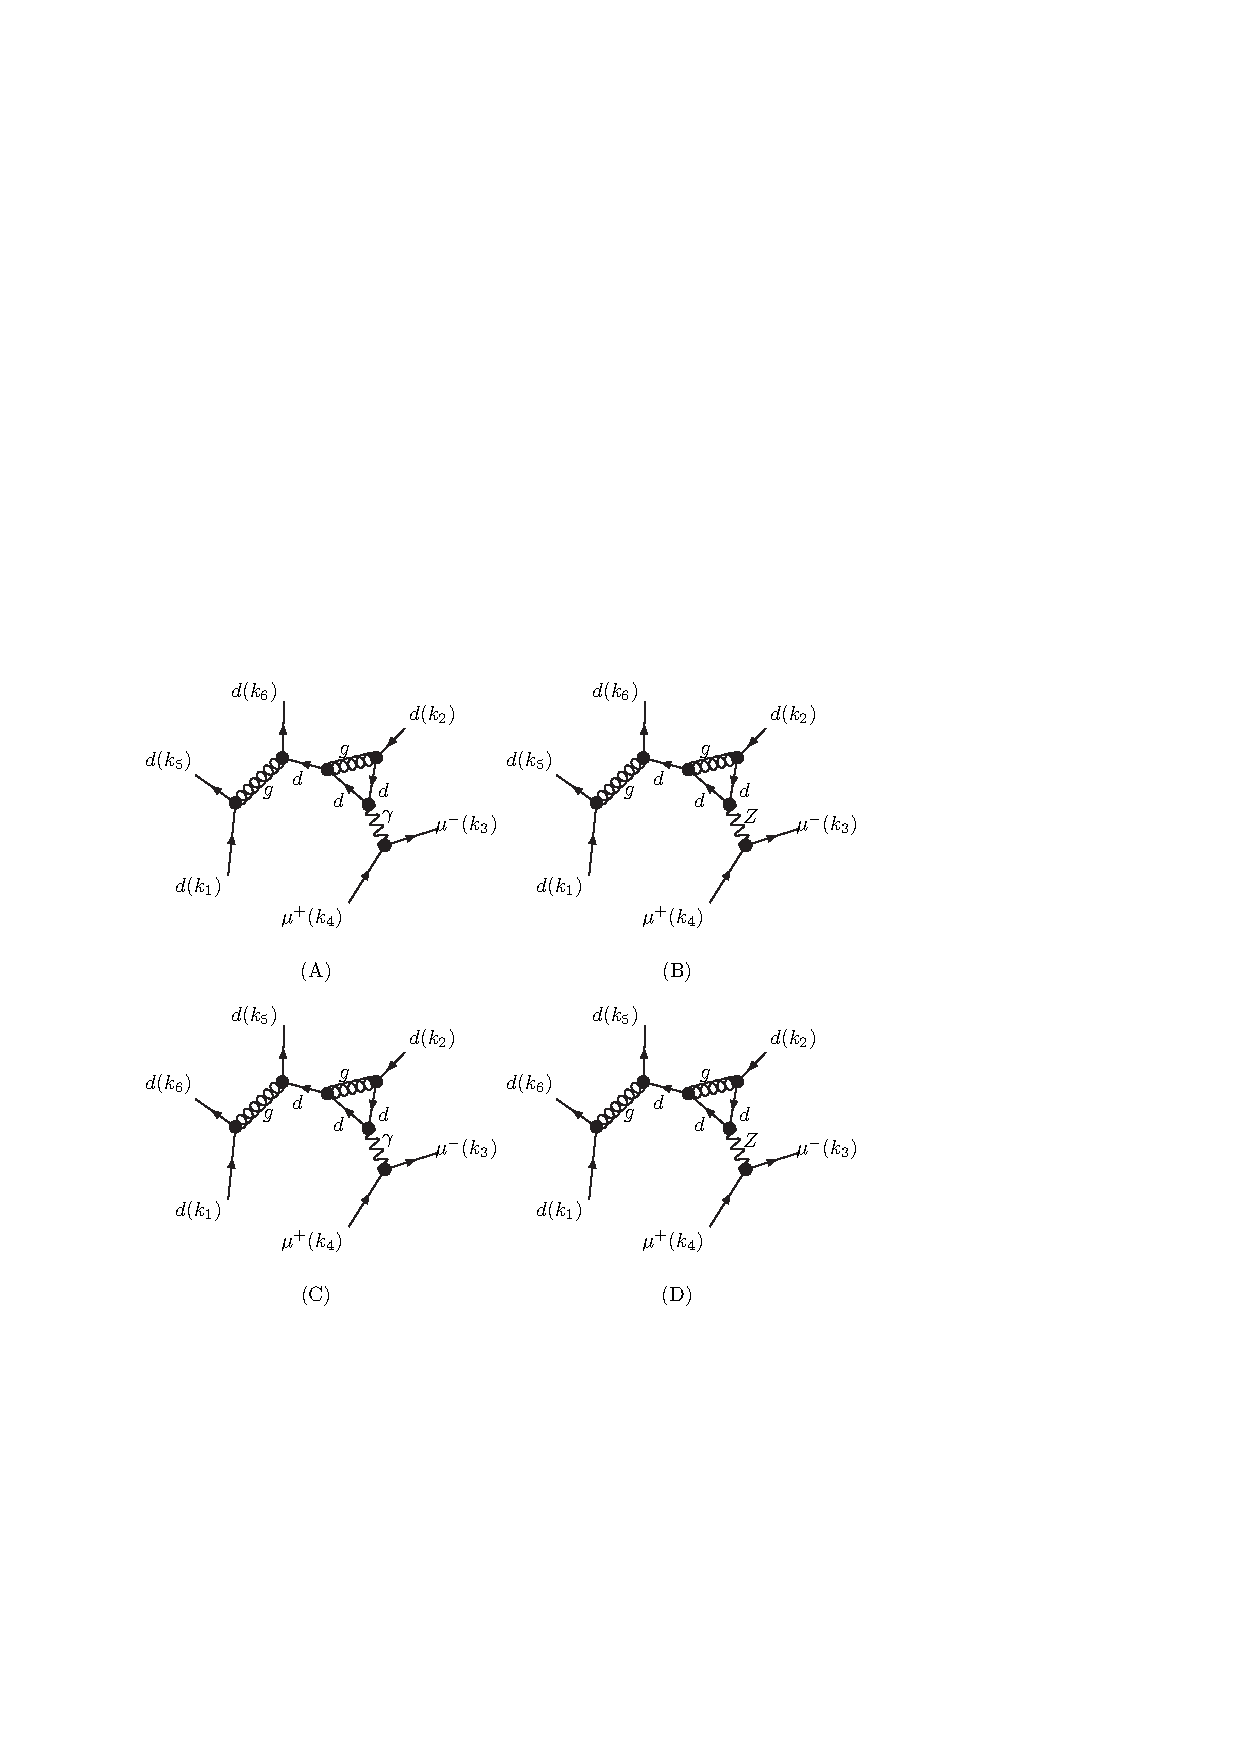
\includegraphics[width=1.0\textwidth]{diagsum1.pdf}
\caption{Example of diagrams sharing a common tree part, which are 
summed when the \texttt{diagsum} option is set to \texttt{diagsum=true}.}
\label{fig:diagsum_tree}
\end{figure} 

\begin{figure}[htb]
\centering
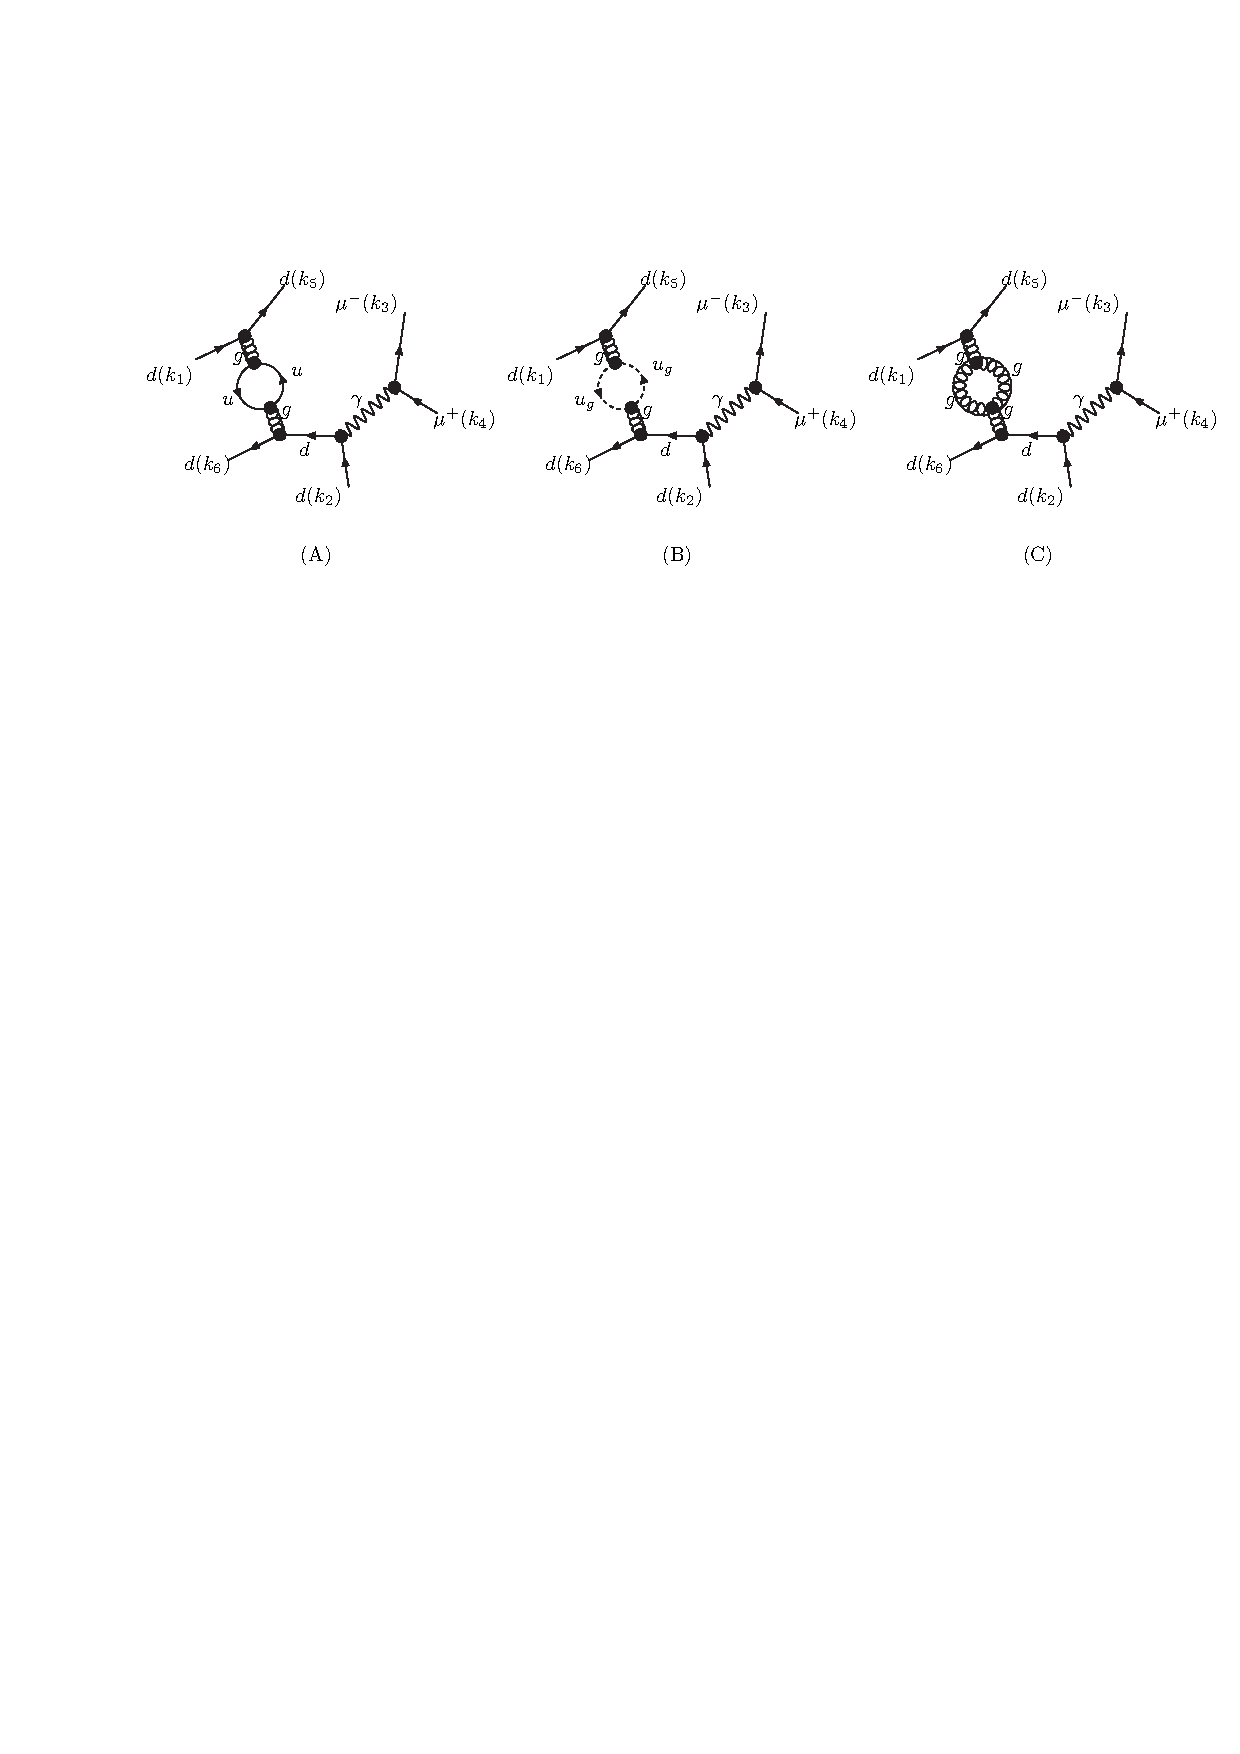
\includegraphics[width=1\textwidth]{diagsum2.pdf}
\caption{Example of diagrams sharing a common loop propagator, 
but with different particle content in the loop, which are summed when
the \texttt{diagsum} option is set to \texttt{diagsum=true}.}
\label{fig:diagsum_particle}
\end{figure} 


When the option \texttt{diagsum} is active (the default behaviour), diagrams which differ only by
a propagator external to the loop, as is the case e.g. for the
$Z/\gamma^\star$ propagator in QCD corrections to the production of
$Z+$jets, are summed together before being processed
by \form{}. Similarly, diagrams which differ only by an external tree
part, but which share exactly the same set of loop propagators, are
summed together prior the algebraic manipulation. An example is shown
Figure~\ref{fig:diagsum_tree}. Finally, diagrams which share the same
set of propagators, but have different particles circulating in the
loop, as shown in Figure~\ref{fig:diagsum_particle}, are also summed
into one ``meta-diagram''. The default setting for this option is \texttt{diagsum=true}.


\subsection*{Grouping of Tree-level Diagrams}

By default the expressions of all tree-level diagrams are grouped into one
file. This has the advantage that subexpressions which appear in several
tree-level diagrams can be reused across the amplitude. The option to turn of this feature is not available anymore as of version 3.0.

\section{Numerical polarisation vectors}
\label{sec:numpolvec}
The use of numerical polarisation vectors for massless gauge bosons
(gluons, photons) is activated by default.  This means that the
various helicity configurations for the massless bosons will be
evaluated numerically, based on the same code, rather than producing
separate code for each helicity configuration.  In order to switch off
this default setting,
for example if the user would like to 
optimize the choice of reference vectors for each helicity configuration,
the option \texttt{polvec=explicit} should be given in the process card 
\texttt{process.in}.
In this case, \gosam{} will choose explicit reference vectors automatically.
If the user wants to specify his/her preferred reference vectors, 
this can be done using the option \texttt{reference-vectors=\ldots}
in the process card.

\section{The extension \texttt{derive} ... is not an extension anymore}
\label{sec:derive}

The \texttt{derive} feature generates code to access the tensor coefficients
of each diagram or group of diagrams individually. It improves both the speed and the precision of tensorial reconstruction and makes connection to other reduction methods. It had been available as an option already in \gosam-1.0 and has been promoted to be used by default in the context of  tensorial reconstruction~\cite{Heinrich:2010ax} in \gosam-2.0. As of version 3.0 it is an integral part of the code and not an extension anymore. Both the keyword \texttt{derive} and its opposite \texttt{noderive} are therefore no valid options for \texttt{extensions} anymore.

The idea behind it is to compute the numerator $\mathcal{N}(\hat{q})$ 
from a Taylor series
\begin{equation}
\mathcal{N}(\hat{q})=\mathcal{N}(0)
+ \hat{q}^\mu
  \frac{\partial}{\partial\hat{q}_\mu}\mathcal{N}(\hat{q})\vert_{q=0}
+ \frac1{2!}\hat{q}^\mu\hat{q}^\nu
  \frac{\partial}{\partial\hat{q}_\mu}
  \frac{\partial}{\partial\hat{q}_\nu}
  \mathcal{N}(\hat{q})\vert_{q=0} + \ldots
\end{equation}
In this form one can read off a one-to-one correspondence between derivatives at
$\hat{q}=0$ and the coefficients of the tensor integrals.

%\paragraph{Implementation.}
At a technical level, 
the files \texttt{helicity*/d*h*l1d.f90} contain the routines
\texttt{derivative($\mu^2$, [$i_1$], [$i_2$],\dots)} and\\
\texttt{reconstruct\_d*(coeffs)}, where the latter is only generated in
conjunction with the extension \texttt{golem95}, and \texttt{coeffs} is
a type which comprises all coefficients of a diagram of a certain rank.
The number of optional indices $i_1$, $i_2$, \dots 
determine which derivative should be returned. The subroutine
\texttt{reconstruct\_d*} also takes into account the proper symmetrisation.

\section{Customization}\label{sec:Customization}
\paragraph{Runtime parameters.}
Many settings can be changed without recompiling the code, by
creating and modifying a file \texttt{matrix/param.dat}.
This file has a very simple format:
\begin{itemize}
\item Lines starting with a comment character (`\texttt{!}', `\texttt{\#}', `\texttt{;}')
      in the first column and blank lines are ignored.
\item All other lines have the format
\begin{lstlisting}[style=in]
name = float
# or
name = float, float
\end{lstlisting}
      where the first line defines a real number and the second
      line defines a complex number, and \texttt{name} is a defined
      parameter.
\item Whitespace is ignored but must not appear inside names or
      literals. Physical lines can not be continued nor can
      multiple entries appear on one line.
\end{itemize}
The list of recognized names can be found in the file
\texttt{common/model.f90}. 
With the built-in Standard Model file (\texttt{sm}) one
can re-set, for example, the value for the Higgs mass by 
\texttt{mH = 125.5}.
All model constants that have not been specified as zero or one
can be set in this way. 
In addition there are some model independent parameters which can be found in the file 
\texttt{common/config.f90}.

\paragraph{Compile time parameters.}
Other configuration options can be found in the file \texttt{common/config.f90}.
\smallskip
Examples of options contained in \texttt{config.f90} are

\begin{longtable}{r p{0.6\textwidth}}
\texttt{ki} & the floating point kind used throughout the calculation, the default is double precision.\\
\texttt{logfile} & an integer specifying the output unit to which all debug output (if activated) is directed. The default is 19. If no file is associated to the unit by means of the \texttt{open} statement in the Fortran code calling the process library the output is written to \texttt{fort.<logfile>}. See the file \texttt{test.f90} in the \texttt{matrix} subdirectory for an example how to write the debug output into a file of your choice.\\
\texttt{debug\_lo\_diagrams} & controls if information about the
    tree level diagrams is written to the debug logfile (see \texttt{logfile} above).\\
\texttt{debug\_nlo\_diagrams} & controls if information about the
    loop-diagrams is written to the debug logfile (see \texttt{logfile} above).\\
\texttt{include\_eps\_terms} & controls if
    terms of order $\varepsilon$ multiplying
    poles are taken into account. (only relevant when \texttt{r2=implicit}, see Appendix~\ref{app:r2})\\
\texttt{include\_eps2\_terms} & controls if
    terms of order $\varepsilon^2$ multiplying
    double poles are taken into account. (only relevant when \texttt{r2=implicit}, see Appendix~\ref{app:r2})\\
\texttt{include\_color\_avg\_factor} & controls if the color averaging
    factor for inital state partons is multiplied to the final result.\\
\texttt{include\_helicity\_avg\_factor} & controls if the helicity averaging
    factor for inital state particles is multiplied to the final result.\\
\texttt{include\_symmetry\_factor} & controls if the symmetry
    factor for identical final state particles
    is multiplied to the final result. \\
\texttt{tens\_rec\_by\_derivatives} & controls whether the tensorial reconstruction method is used. (only relevant when using \golemVC{})
\end{longtable}

\section{Drawing the Feynman diagrams}
In order to print out the diagrams the makefile contains the target
\texttt{doc} which produces the file \texttt{process.pdf}.
We use \LaTeX{} plus the package \textsf{axodraw}~\cite{Vermaseren:1994je}
to create the graphical representation.

The layout of the diagrams is determined by the algorithm used in
\textsf{feynMF}~\cite{Ohl:1995kr}, modelling the propagators by springs.
The implemented algorithm works in two steps: first, the topology is
constructed by ordering the external legs such that the diagram can
be drawn as a planar graph. The coordinates $e_k$
of the external legs are
fixed along a contour around the drawing area.
In a second step the remaining degrees of freedom, the coordinates
of the vertices $v_i=(x_i, y_i)$, are fixed by minimizing the Lagrangian
\begin{equation}
L(v_1, \ldots, v_n; e_1, \ldots, e_N) =
 \frac14\sum_{i,j=1}^n t_{ij}\left(v_i-v_j\right)^2
+\frac12\sum_{i=1}^n\sum_{k=1}^N\lambda_{ik}\left(v_i-e_k\right)^2
\end{equation}
Here, $n$ is the number of vertices and $N$ is the number of external
legs.
Minimization of the Lagrangian leads to a system of linear equations, which
can easily be solved.
\begin{align*}
&\frac{\partial L}{\partial v_r}=0\\
\Leftrightarrow&
 \frac12\sum_{i,j=1}^n t_{ij}\left(v_i-v_j\right)
     \cdot\left(\delta_{ir}-\delta_{jr}\right)
+\sum_{i=1}^n\sum_{k=1}^N\lambda_{ik}\left(v_i-e_k\right)
     \cdot\delta_{ir}=0\\
\Leftrightarrow&
M_{rj}v_j\equiv
 \sum_{j=1}^n t_{rj}\left(v_r-v_j\right)
+\left(\sum_{k=1}^N\lambda_{rk}\right)v_r
=\sum_{k=1}^N\lambda_{rk}e_k
\end{align*}
In the last step we used the symmetry of $t_{ij}$.
The matrix $M$ can be written as
\begin{equation}
M_{rc}=\left\{\begin{array}{ll}
\left(\sum_{i\neq r}t_{ri}\right)+
\left(\sum_{k=1}^N\lambda_{rk}\right),&
r=c\\
-t_{rc},&\text{otherwise}
\end{array}\right.
\end{equation}

The symbol $t_{ij}$ is the sum of the spring constants of all
propagators connecting vertices $i$ and $j$; similarly, $\lambda_{ik}$
is the spring constant of the leg $k$ if it is connected to vertex $i$
and zero otherwise.

\section{Import of model files}
\label{sec:model}

The \gosam{}-\gosamversion{} package comes with the built-in model files 
\texttt{sm}, \texttt{smdiag}, \texttt{smdiag\_mad}, \texttt{smehc}, \texttt{smdiagehc},
\texttt{sm\_complex}, \texttt{smdiag\_complex}, 
where the latter two are needed in the case of complex masses and couplings, 
see Section~\ref{sec:complexmasses}. 
The model files \texttt{smdiag\_mad} contain some \texttt{MadGraph5} specific settings, while
the model files \texttt{smehc} and \texttt{smdiagehc} contain the effective Higgs-gluon couplings.

Other models can be imported most easily in the UFO (Universal Feynman Output)~\cite{Degrande:2011ua,Darme:2023jdn} format.
The model import in the UFO format can be used in the standalone as well as the OLP 
mode of \gosam, where both the BLHA1 and BLHA2 standards are supported for the syntax of the model import.

In order to perform calculations in an EFT like SMEFT or HEFT the user is required to provide the EFT model in the UFO format. See Section~\ref{sec:EFT} for more details.

Examples about how to import model files can be found in the subdirectory 
 \texttt{examples}.

\subsection{Import of a UFO model}\label{sec:UFO}
A model description in the UFO~\cite{Degrande:2011ua,Darme:2023jdn} format consists of a Python package
stored in a directory. In order to import the model into \gosam{} one needs
to set the \texttt{model} variable specifying the keyword \texttt{FeynRules}
in front of the directory name.
For example, if the Python model files for the MSSM are in 
 the directory \\
 \texttt{\$HOME/models/MSSM\_UFO}, the process card must contain the line
\begin{lstlisting}[style=in]
model= FeynRules,$HOME/models/MSSM_UFO
\end{lstlisting}
All parameters of type ``external'' defined in the UFO model's \texttt{parameter.py} file will become available as runtime parameters (see Section~\ref{sec:Customization}). To distinguish them from parameters defined within \gosam directly they are prepended with the prefix \texttt{mdl}. \gosam will try to figure out the correct naming of the strong (electroweak/QED) coupling by checking if the model contains any parameter, external or internal, denoted \texttt{G}, \texttt{GG} or \texttt{GS} (\texttt{E}, \texttt{EE}, \texttt{ee}).

In a UFO model each coupling is assigned a specific order, that is its power wrt. the QCD and/or QED coupling. In general more ``orders'' can be defined in the model, a feature which is useful to distinguish certain sets or classes of couplings. An example for an often used order is \texttt{NP}, which can be used to flag couplings of BSM or EFT origin. \gosam enables the user to make use of this UFO feature by means of the \python filter (see Section~\ref{sec:filter}) \texttt{d.order('order')}, where \texttt{'order'} is a string denoting the name of the order parameter as defined in the UFO, e.g. \texttt{'NP'}. If the user wants to apply a filter based on a specific order, the property \texttt{order\_names} has to be declared in the process configuration file, e.g. \texttt{order\_names=NP}.

\attention{\gosam is not able to handle arbitrarily large UFO models because of the limited buffer available in \qgraf. If the model is too large the user will be prompted a \qgraf error. In that case it might help to comment out vertices not contributing to the process from the UFO model files before starting \gosam.}


\attention{Care has to be taken regarding the sign conventions adopted in the model. In most cases this concerns the convention chosen for the gauge field part of the covariant derivative and the overall sign of the ghost term in the Lagrangian. In both there is a certain freedom and no general consensus exists in the literature. See e.g.~\cite{Romao:2012pq} for a review. The sign chosen for the covariant derivative only manifests itself in the Feynman rules for the vertices and as long as the model files are consistent the matrix elements should be independent of the convention.\footnote{One can convince oneself that the sign will always appear squared. However, there is an exception when considering EFTs. Depending on the definition of the EFT operators it can happen that a sign dependence remains. This dependence can be absorbed into a redefinition of the Wilson coefficients of the concerned operators.} The sign chosen for the ghost terms will in addition appear in the ghost propagator. Since  \gosam relies on an internal implementation of the propagators and does not take them from the UFO model, it is important that the model matches the sign convention of the ghosts considered in \gosam:

\begin{equation*}
   i\Pi_\mathrm{gh}^{ab}(k) = \frac{i\delta^{ab}}{k^2+i\epsilon}\,,
\end{equation*}

which corresponds to $\eta_G=+1$ in the nomenclature of~\cite{Romao:2012pq}. As the chosen sign conventions cannot easily be extracted from the UFO model it is the responsibility of the user to provide a consistent setup.}

\subsection{Import from LanHEP}
\attention{Since by now LanHEP also provides output in the UFO format we recommend using this format over the older LanHEP format.}
In order to use model files generated by LanHEP the following steps
have to be taken:
\begin{enumerate}
\item When generating the tables using LanHEP, one should include the
   following option to ensure that the generated tables have the correct
   headings\footnote{\gosamv{} relies on the column names rather than
   some specific order.}. The number of spaces in the column headers are
   irrelevant as long as the columns are wide enough to contain the
   respective values.
\begin{lstlisting}[style=in]
   prtcformat
      fullname: '  fullname  ',
      name:     '  name   ',
      aname:    '  aname  ',
      spin2:    '  spin2  ',
      mass:     '  mass  ',
      width:    '  width  ',
      color:    '  color  ',
      aux:      '  aux  ',
      texname:  '      texname      ',
      atexname: '     atexname      ',
      pdg:      '  pdg   '.
\end{lstlisting}
\item If the model file is not already equipped with pdg codes
   the user might want to use the \verb!prtcprop! command in
   LanHEP to add the relevant codes.
\item In the setup file, one needs to specify the model as a pair
   of path and integer number. If the table files are under the directory
   \texttt{lanhep/ued/} in the tables \texttt{func7.mdl}, \texttt{lgrng7.mdl},
   \texttt{prtcls7.mdl} and \texttt{vars7.mdl}, the correct statement in
   the setup file would be
\begin{lstlisting}[style=in]
   model=lanhep/ued, 7
\end{lstlisting}
\end{enumerate}

\attention{Note that the use of user defined functions (\texttt{external\_func} in LanHEP) is not supported any longer.}


\subsection{Propagators for spin-2 particles}
\label{sec:spin2}

The propagator for massive spin-2 particles can be split into two parts
\begin{align}
	i \Delta_{\mu\nu,\rho\sigma}(k,m_{\vec n}) =  \underbrace{\frac{i}{k^2-m_{\vec n}^2 + i\epsilon}}_{D(k^2,m_{\vec n})} B_{\mu\nu,\rho\sigma}(k,m_{\vec n})\;,
\end{align}
where $B_{\mu\nu,\rho\sigma}$ carries the Lorentz structure
\begin{align}
	B_{\mu\nu,\rho\sigma}(k,m) =&
	             \left(\eta_{\mu \rho} - \frac{k_\mu k_\rho}{m^2}\right) 
		     \left(\eta_{\nu \sigma} - \frac{k_\nu k_\sigma}{m^2}\right)\notag \\
         &  + \left(\eta_{\mu \sigma} - \frac{k_\mu k_\sigma}{m^2} \right)
		     \left(\eta_{\nu \rho} - \frac{k_\nu k_\rho}{m^2}\right) \notag \\
         &  - \frac23  
	   \left(\eta_{\mu \nu} - \frac{k_\mu k_\nu}{m^2}\right)
	   \left(\eta_{\rho \sigma} - \frac{k_\rho k_\sigma}{m^2}\right)\;.
\end{align}

If all particles attached to the propagator are on-shell, 
the mass dependent terms in $B_{\mu\nu,\rho\sigma}(k,m)$ drop out.
Further, if the on-shell condition is not always fulfilled, 
it turned out in phenomenological applications that the impact of the mass dependent terms is numerically 
negligible\,\cite{Gleisberg:2003ue,Greiner:2013gca}
and therefore we did not include them in our implementation
in order to avoid an enormous proliferation of terms.
In this case the summation over the graviton states  in $D(s,m_{\vec n})$, leading to
\be
D(s) = \sum_{\vec n} \frac{i}{s-m_{\vec n}^2 + i \epsilon}\;,
\ee
can be performed independently from the  $B_{\mu\nu,\rho\sigma}$ part carrying the Lorentz structure.
Further, in  models with large extra dimensions (LED),
 we can use the assumption that the widths of the KK modes are negligible, 
as the dominant effects come from the almost on-shell production of KK modes, 
and that the discrete spectrum of the KK  modes can be approximated by an
integral over a mass density, as the  KK modes are very contiguous.
%\,\cite{Han:1998sg,Giudice:1998ck}. 
The density as a function of the mass $m_{\vec n}$ is given by
\be
\rho(m_{\vec n})=\frac{R^{\delta}m_{\vec n}^{\delta - 2}}{(4\pi)^{\delta/2}\Gamma(\delta/2)}\;,
\ee
where $\delta$ is the number of extra dimensions, leading to \,\cite{Han:1998sg}
\begin{align}
	D(s) \to  \int_0^{M_S} d\,m_{\vec n}^2\,
	\frac{i\,\rho(m_{\vec n})}{s-m_{\vec n}^2+ i \epsilon}
	= \begin{cases} \frac{ s^{\delta/2-1}}{2M_{s}^{\delta + 2} G_N } \left( \pi + 2 i \, I(\frac{M_S}{\sqrt{s}}) \right) & \text{for\ } s>0 \\
		\frac{ (-s)^{\delta/2-1}}{2M_{s}^{\delta + 2} G_N} (-2i)\, I_E(\frac{M_S}{\sqrt{-s}}) & \text{for\ } s<0 
	\end{cases}
	\label{eq:propagator}
\end{align}
with 
\begin{align}
	I(x) = \begin{cases} - \sum_{k=1}^{\delta/2-1} \frac1{2k} x^{2k} - \frac12 \log(x^2-1)& \text{if\ } \delta \text{ even} \\
		- \sum_{k=1}^{(\delta-1)/2 } \frac{1}{2k-1} x^{2k-1} + \frac12 \log\left( \frac{x+1}{x-1} \right) & \text{if\ } \delta \text{ odd}
	\end{cases}
\end{align}
and
\begin{align}
	I_E(x) = \begin{cases} (-1)^{\delta/2 + 1} \left( \sum_{k=1}^{\delta/2-1} \frac{(-1)^k}{2k} x^{2k} + \frac12 \log(x^2+1)  \right) 
		& \text{if } \delta \text{ even} \\
		(-1)^{(\delta-1)/2} \left(   \sum_{k=1}^{(\delta-1)/2 } \frac{(-1)^k}{2k-1} x^{2k-1} + \frac12 \tan^{-1}(x) \right)   & \text{if } \delta \text{ odd} \,.
	\end{cases}
\end{align}
The UV cutoff $M_S$ is introduced as the effective theory approach loses its validity beyond the scale $M_S$.


\gosam{} supports spin-2 propagators with the \texttt{customspin2propagator} extension which
needs to be enabled in the process card by \\
\texttt{extensions=customspin2propagator}.

The extension works only if the model is imported from an UFO file. 
The latter can  be adjusted to the needs of the particular model the 
user would like to consider by editing the file \texttt{custompropagator.f90}
in the subdirectory \texttt{common}. 
In order to generate the latter file,
the spin-2 particle which should get a customized propagator needs to have a
separate attribute 'CustomSpin2Prop' in the UFO file with a non-vanishing
value:\\
Excerpt of \texttt{LED\_UFO/particle.py} with a customized propagator:
\begin{lstlisting}[style=py]
    Gr = Particle(pdg_code = 9000006,
                  name = 'Gr',
                  # ...
                  CustomSpin2Prop = 1
                 )
\end{lstlisting}
Then \gosam{} generates a the file \texttt{common/custompropagator.f90} where the user needs
to adapt the \texttt{customSpin2Prop} subroutine.
Beside the squared momentum, the \texttt{customSpin2Prop} subroutine also receives the
mass of the corresponding spin-2 particle as an argument, which
can be used to distinguish between multiple spin-2 particles if necessary.
The tensorial part of the spin-2 propagator, $B_{\mu\nu,\rho\sigma}(k,m_{\vec n})$, is treated separately 
and should not be modified.  If the user would like to modify it, we refer to the  documentation in 
section 6.3 of \texttt{src/form/lorentz.pdf} in the \gosam{} tarball.
